%! TEX root = **/000-main.tex
% vim: spell spelllang=en:

\section{Extrapolation}%
\label{sec:extrapolation}

It is crucial that we choose an extrapolation method which benifits from the specific properties of our system and solver.
Due to the time constraint on this project we haven't investigated the stability or error bound properties for the extrapolation methods.
While this would be an interesting area to do further research in, we chose methods for which we can safely ignore these properties.
Neuro-VISOR uses the Semi-Implicit Backward Difference 2 method\cite{neuroVISOR}, so linear and quadratic extrapolation are both good options.
To minimize the runtime and memory usage of the extrapolation we've chosen to implement linear extrapolation.

\begin{figure}[H]
    \centering
    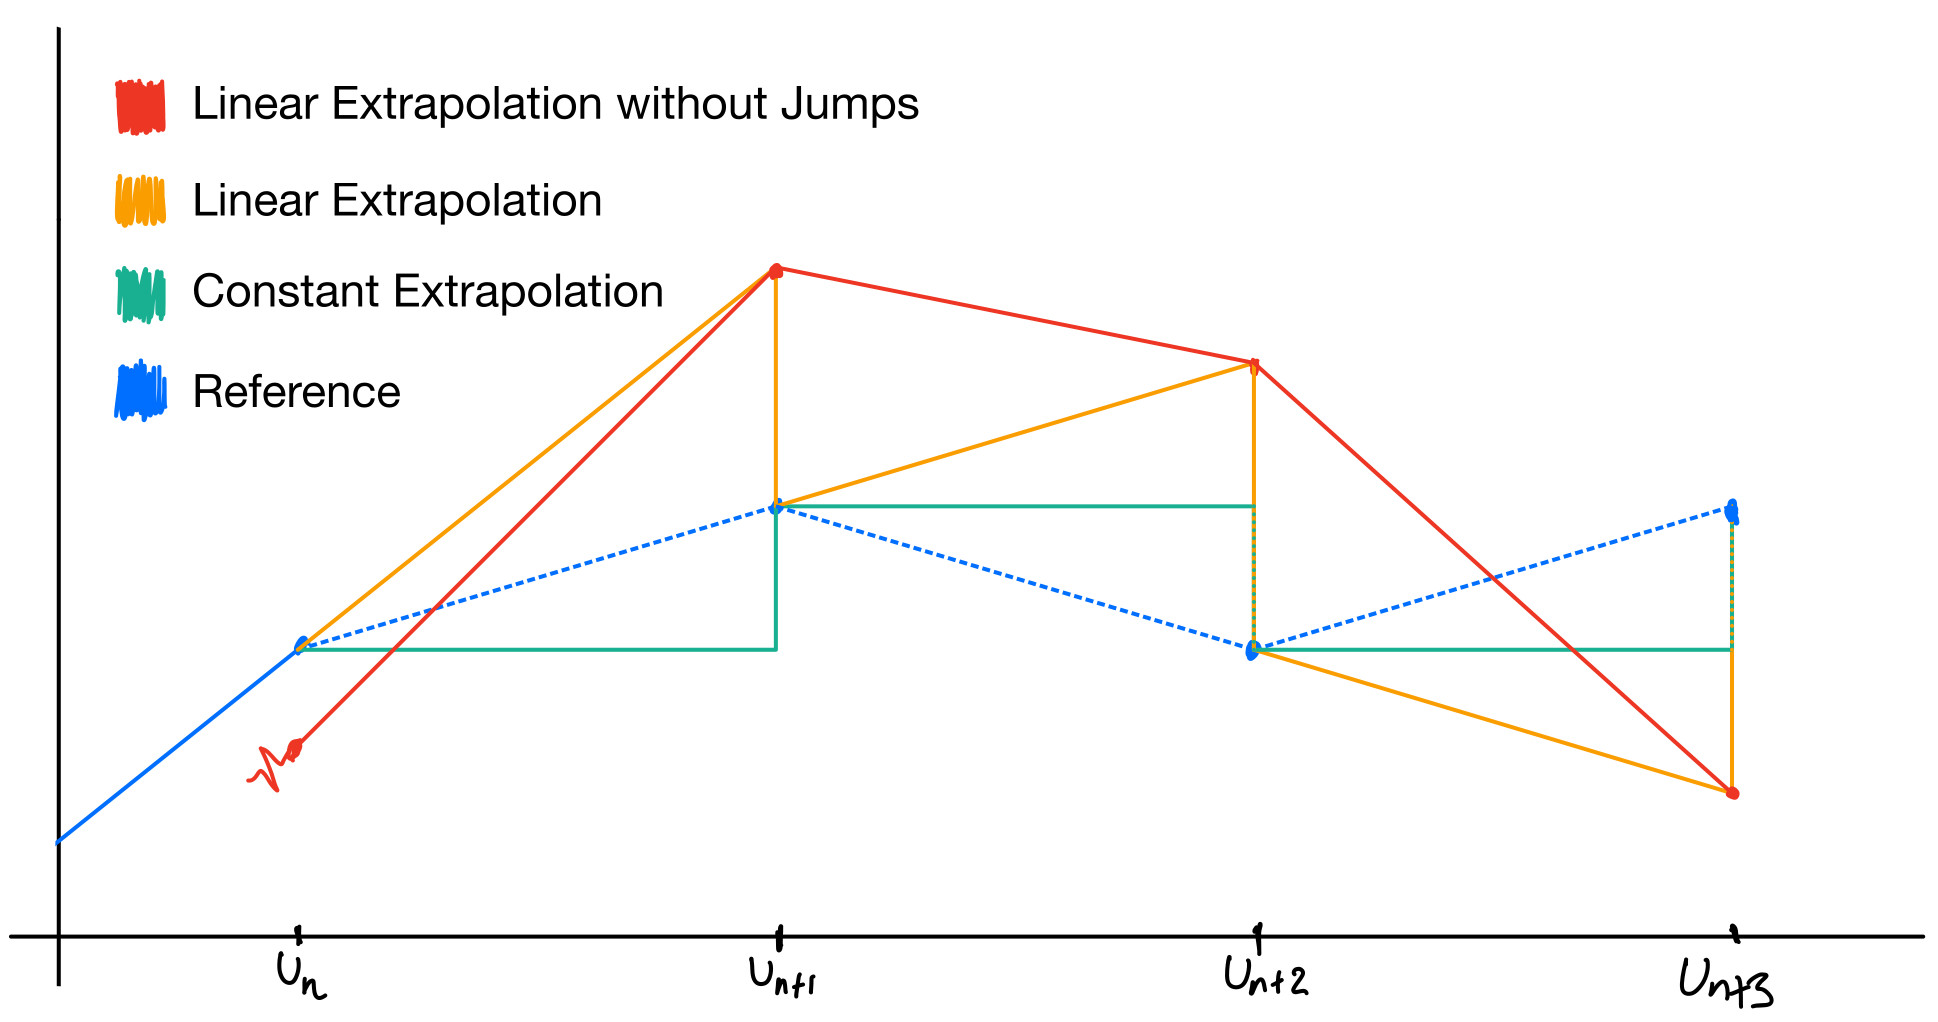
\includegraphics[width=1.0\linewidth]{extrapolationOptions}
    \caption{Linear Extrapolation Methods}%
    \label{fig:extrapMethods}
\end{figure}

\subsection{Optimal Methods}%
\label{sub:optimal_methods}

Linear extrapolation requires a linear function defined in terms of the previous data points.
We can think of linear extrapolation as a family of linear functions $\hat{u}_t : \mathbb{N} \to \mathbb{R}$ parameterized by $t \in [0,1]$ where $\hat{u}_t(n)$ is the point to which the point $u_n$ has moved at time $t$.
The naive definition would be $\hat{u}_t(n) = u_n$, which we will call the constant function and which can be seen in \cref{fig:extrapMethods} in green.
Technically Neuro-VISOR implements this when the visualization updates more frequently than the simulation.
Another option is $\hat{u}_t(n) = (1-t)u_n + t(2u_n - u_{n-1})$, which corresponds to yellow in \cref{fig:extrapMethods}.
A third option is $\hat{u}_t(n) = (1-t)(2u_{n-1} - u_{n-2}) + t(2u_n - u_{n-1})$, which can be seen as red in \cref{fig:extrapMethods}.


Linear extrapolation requires a linear function defined in terms of the previous data points.
For the following definitions, let $u_n$ be the values of the simulation at step $n$.
As seen in \cref{fig:extrapMethods}, there are multiple ways of defining the linear function.
The naive way would be to use the constant function equal to the most recent data point.
An example of this can be seen in \cref{fig:extrapMethods} as the green option.
Technically Neuro-VISOR implements this when the visualization updates more frequently than the simulation.
Another option is to use the tangent line defined by the previous two data points.
This corresponds to the yellow option in \cref{fig:extrapMethods}.
A third option is to use the slope between the previous two data points and the point along the previous extrapolation which coincides with the time of the most recent data point.
This can be seen in \cref{fig:extrapMethods} in red.

As mentioned in the introduction, the goal of this project is to improve the visualization and user experience of the program during unexpected slow downs.
While this is not rigorously defined, we will suppose abrupt jumps decrease the user's experience.
This seems like a reasonable heuristic as abrupt jumps are jarring and make it difficult to follow the simulation.
The naive line results in a jump whenever a new data point is calculated unless the system is constant.
The tangent line also results in a similar number of jumps, but the jumps will generally be smaller than the naive line.
Because of this, the tangent line is strictly better for our use case.
The third option doesn't contain any jumps.
However, since it doesn't jump to the most recent data point the error bounds accumulate.
For example, \cref{fig:l1} shows plots of the L1 norms for the same configuration save one using linear extrapolation with jumps and the other using linear extrapolation without jumps.
The L1 graph of the linear extrapolation with jumps has a characteristic sawtooth shape due to it's value being set to the real data point every ten steps.
On the other hand, the L1 graph of the linear extrapolation with jumps will approach the value the other graph approaches before each jump due to it's definition.
The shape of \cref{fig:l1} is similar with larger troughs due to the starting point not being an actual value point.
These are the two methods that are implemented in our codebase.

\begin{figure}[H]
    \centering
    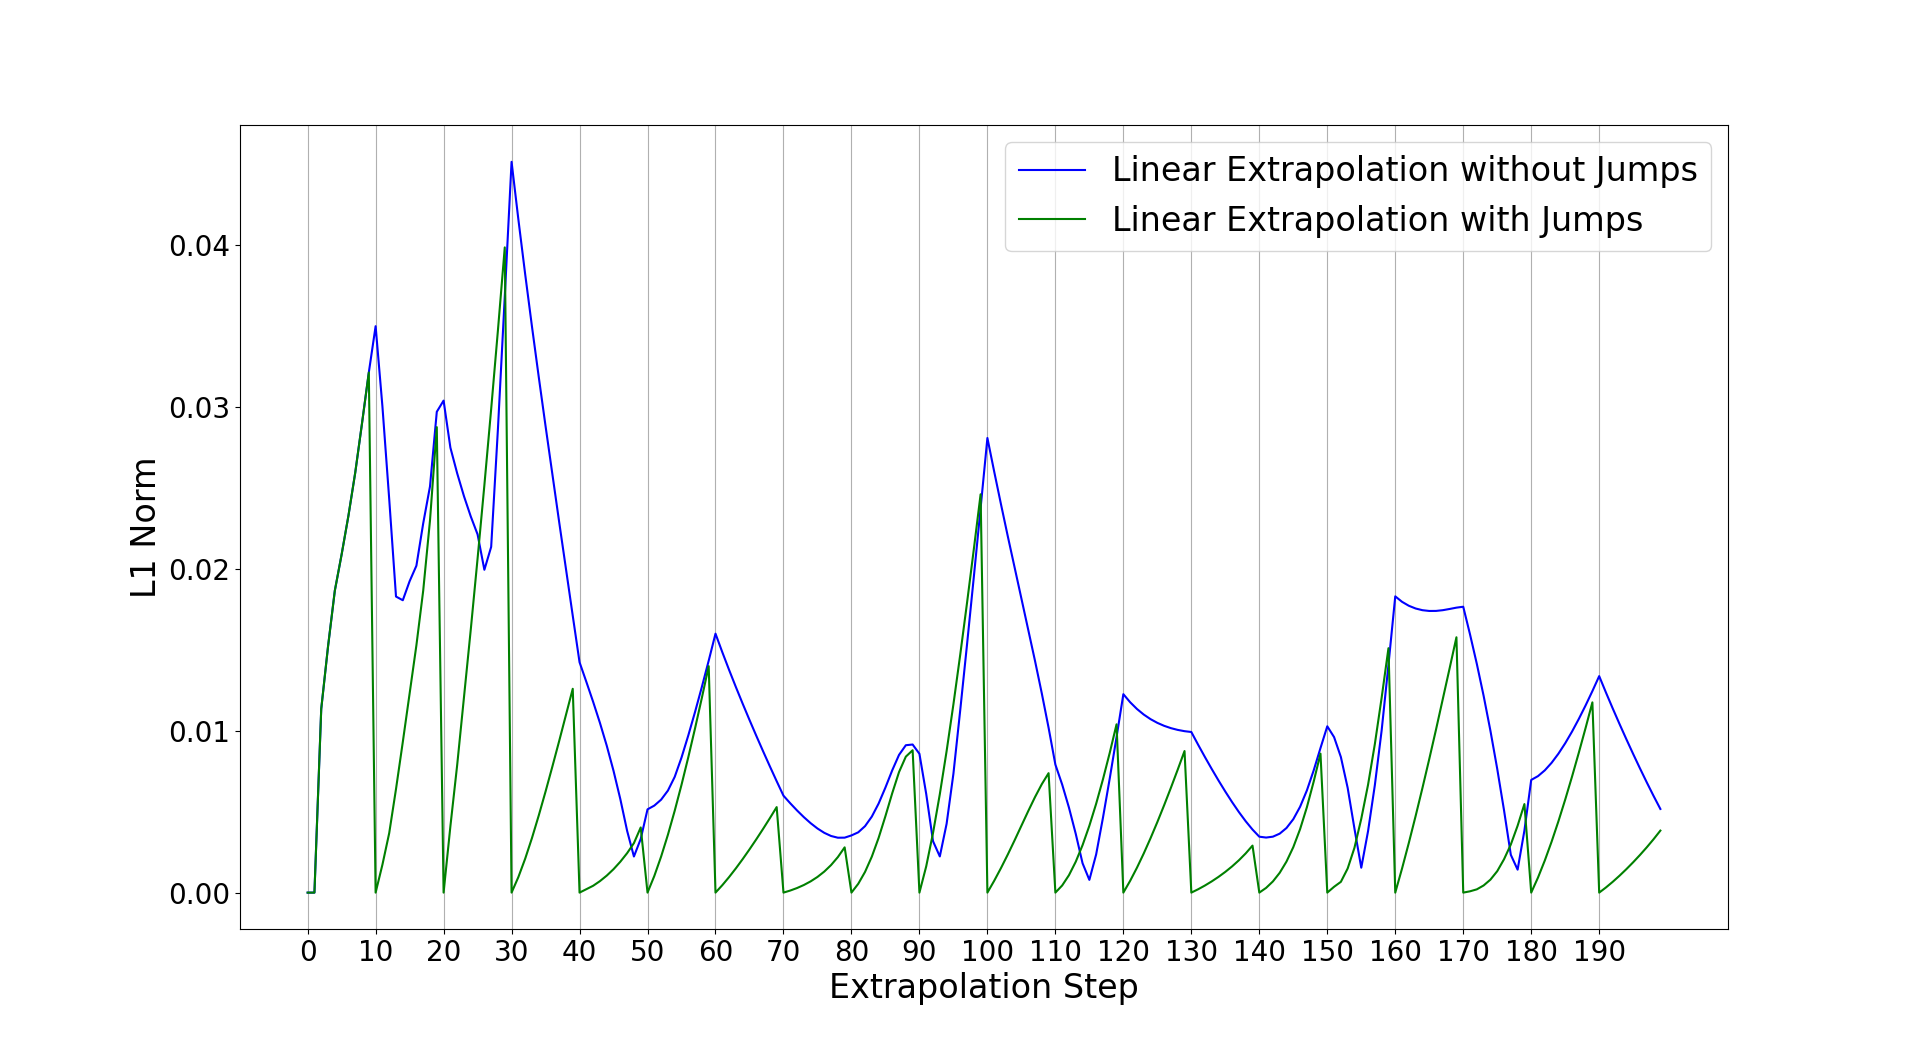
\includegraphics[width=1.0\linewidth]{endpointFull_both}
    \caption{L1 Norms for Linear Extrapolations}%
    \label{fig:l1}
\end{figure}


\subsection{Next Steps}%
\label{sub:next_steps}

The two extrapolation methods that we have focused on are not necessarily the best options.
They both have their pros and cons, however there may be ways of defining linear functions which don't contain jumps but have smaller error bounds.
For example, one could cap the distance between the point used and the previous data point.
Another way could be to define the slope using both the tangent slope and the distance between the starting point and previous data point.
This is an interesting area for future study, especially showing rigorous results in this area and exploring non-linear options.
